\section{Resultados}
\label{sec:resultados}
% S03-10 (#176): RQ01 a RQ04 e classificação C1; notebooks em Lab03/analise/
% (#167, #168, #169). RQ05 a RQ07 entram nas subseções seguintes (#177, #178).

Os resultados referem-se aos 500 repositórios da amostra final
(Seção~\ref{sec:metodologia}). Cada métrica é resumida pela mediana e pelo
intervalo interquartil (IQR) entre repositórios, apenas com os valores
válidos; ausências não são tratadas como zero. A Tabela~\ref{tab:resumo-rq}
reúne os resumos, e as Figuras~\ref{fig:rq01-rq02} e~\ref{fig:rq03-rq04}
mostram as distribuições.

\begin{table}[ht]
\centering
\caption{Resumo das métricas entre repositórios}
\label{tab:resumo-rq}
\small
\begin{tabular}{llrrr}
\hline
RQ & Métrica (unidade) & $n$ & Mediana & IQR (Q1--Q3) \\
\hline
RQ01 & Frequência de deploy (releases/semana) & 500 & 0,48 & 0,23--1,13 \\
RQ02 & Lead time (a) por release (horas) & 499 & 268 & 91--928 \\
RQ02 & Lead time (b) por commit (horas) & 499 & 303 & 79--1.225 \\
RQ03 & CFR (a) por runs (fração) & 500 & 0,053 & 0,023--0,118 \\
RQ03 & CFR (b) por releases corretivas (fração) & 498 & 0,440 & 0,200--0,727 \\
RQ04 & Tempo de recuperação (horas) & 469 & 2,6 & 1,1--7,2 \\
\hline
\end{tabular}
\end{table}

\begin{figure}[ht]
\centering
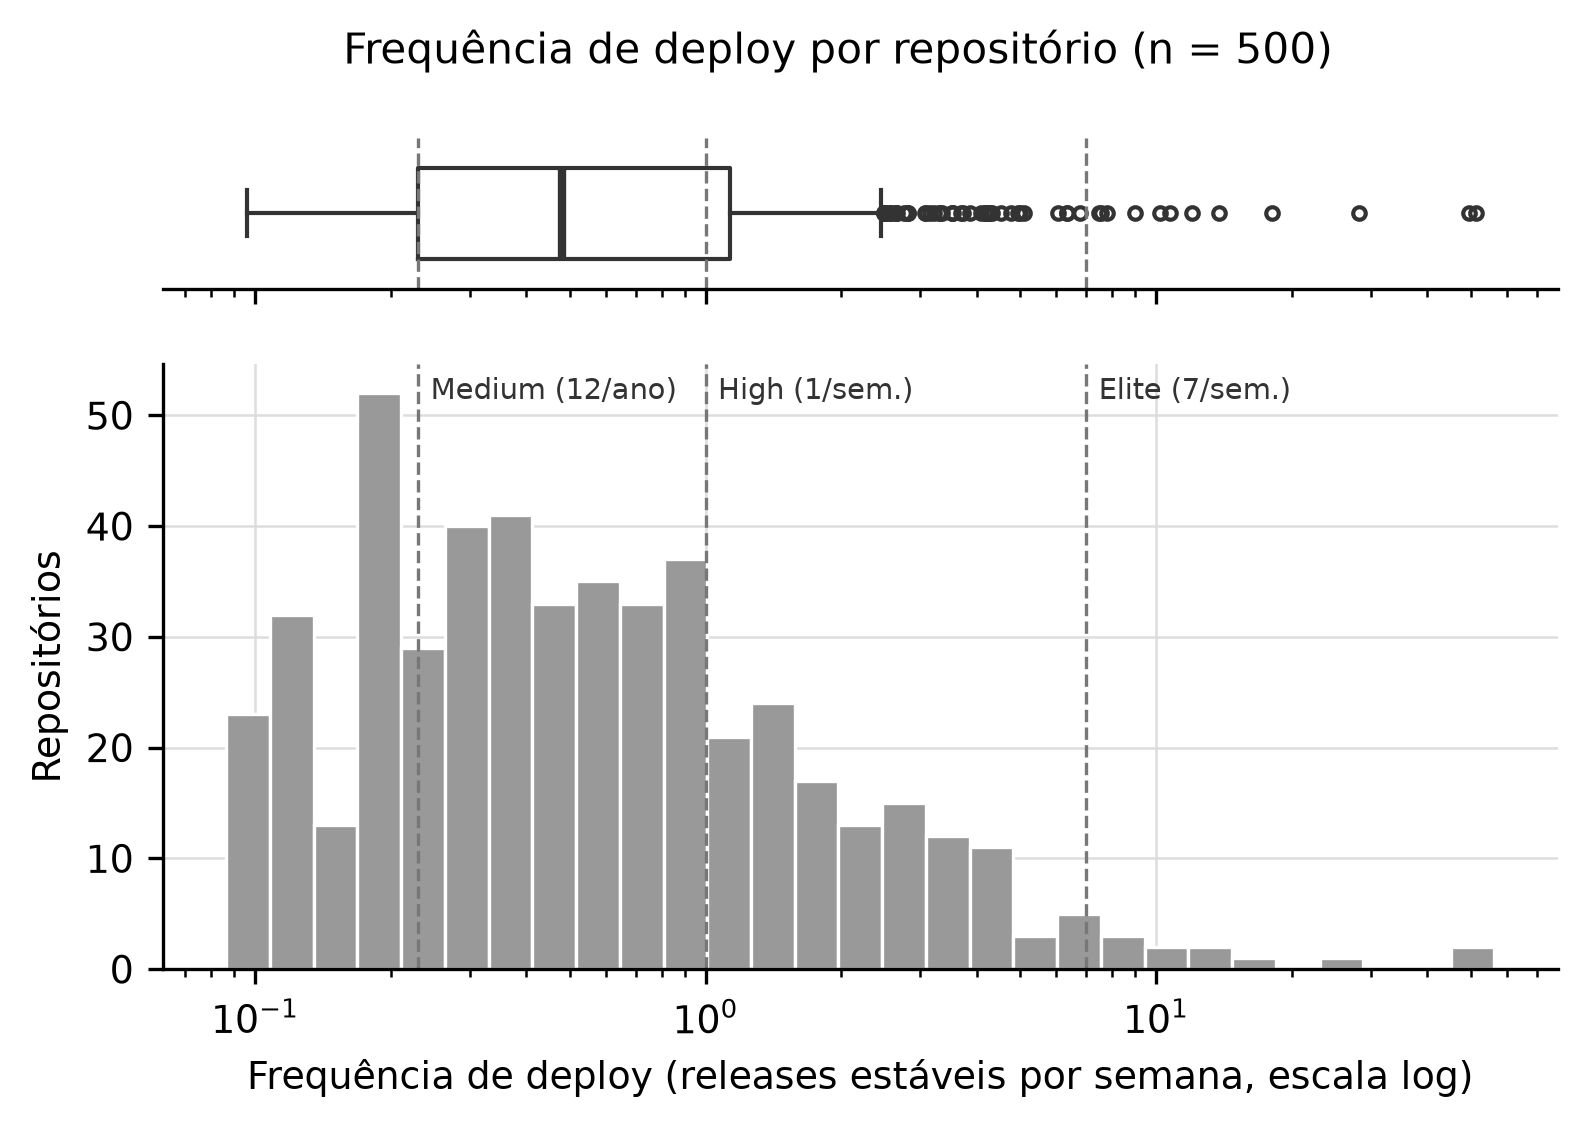
\includegraphics[width=0.49\textwidth]{rq01_frequencia_deploy.png}\hfill
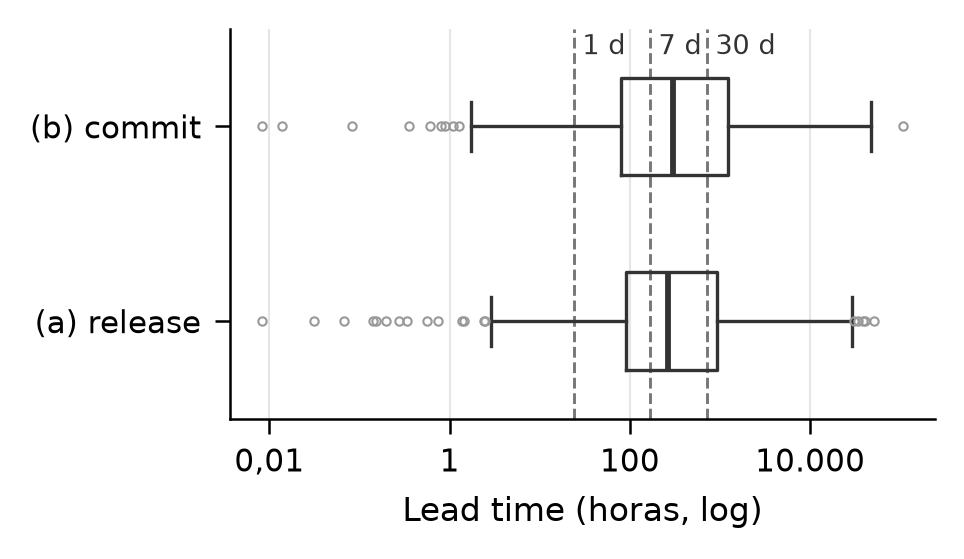
\includegraphics[width=0.49\textwidth]{rq02_lead_time_variantes.png}
\caption{Frequência de deploy (esquerda) e lead time por variante (direita),
em escala logarítmica; linhas tracejadas marcam os cortes DORA}
\label{fig:rq01-rq02}
\end{figure}

\subsection{RQ01 -- Frequência de deploy}
A mediana da frequência de deploy é de 0,48 release estável por semana,
cerca de 2,1 por mês, com IQR de 0,23 a 1,13 por semana. A distribuição é
assimétrica à direita: o máximo chega a 51,3 releases por semana. Em termos
mensais, 24,0\% dos repositórios publicam menos de uma release por mês,
36,6\% entre uma e três, e 39,4\% mais de três.

\subsection{RQ02 -- Lead time}
Há lead time para 499 repositórios; o restante não tem comparação válida
entre releases. Pela variante (a), por release, a mediana é de 268~horas
(11,2 dias), com IQR de 91 a 928~horas. Pela variante (b), por commit, a
mediana é de 303~horas (12,6 dias), com IQR de 79 a 1.225~horas. No mesmo
repositório, a variante (a) é maior que a (b) em 303 casos (60,7\%), menor
em 195 e igual em um; a mediana da razão (a)/(b) é 1,29. A mediana entre
repositórios de (a) fica abaixo da de (b) porque a variante (b) tem cauda
superior mais longa.

\begin{figure}[ht]
\centering
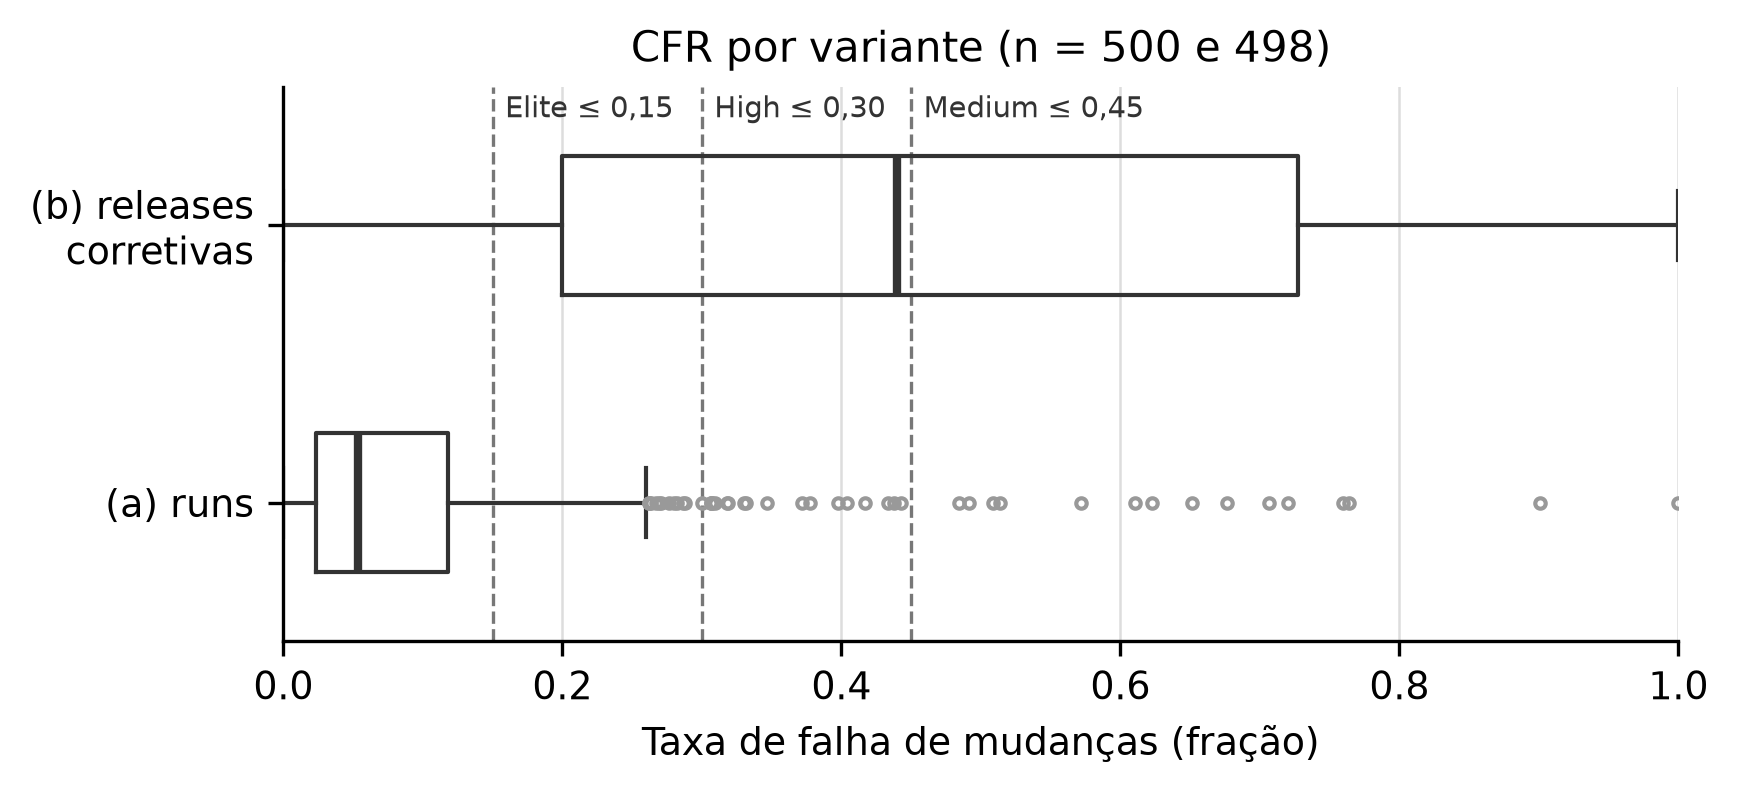
\includegraphics[width=0.49\textwidth]{rq03_cfr_variantes.png}\hfill
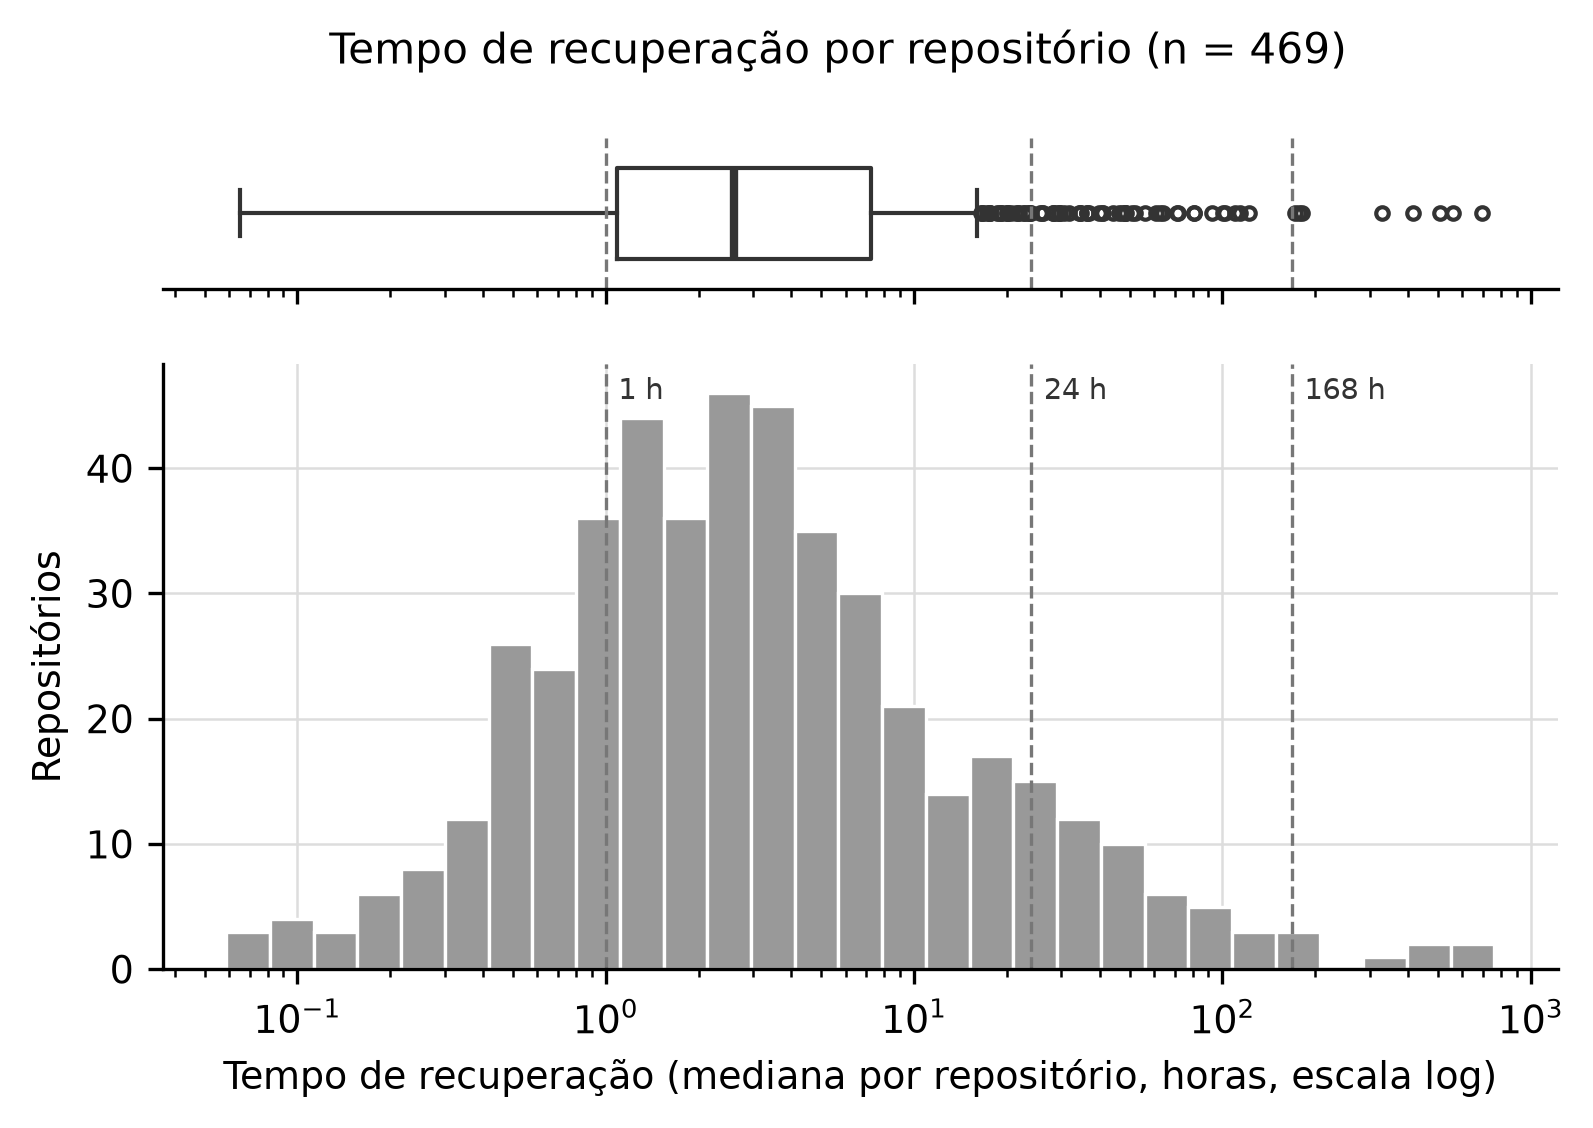
\includegraphics[width=0.49\textwidth]{rq04_tempo_recuperacao.png}
\caption{CFR por variante (esquerda) e tempo de recuperação por repositório,
em escala logarítmica (direita); linhas tracejadas marcam os cortes DORA}
\label{fig:rq03-rq04}
\end{figure}

\subsection{RQ03 -- Taxa de falha de mudanças}
A CFR (a), calculada sobre os runs válidos, tem mediana de 0,053 e IQR de
0,023 a 0,118 nos 500 repositórios. A CFR (b), calculada pela heurística v1
de releases corretivas, tem mediana de 0,440 e IQR de 0,200 a 0,727 em 498
repositórios. A variante (a) é menor que a (b) em 425 dos 498 pares, e
apenas 104 repositórios (20,9\%) ficam na mesma classe DORA pelas duas
variantes. A CFR (b) ainda depende da avaliação da heurística contra os
rótulos de consenso da amostra-ouro.

\subsection{RQ04 -- Tempo de recuperação}
Há episódios recuperados em 469 repositórios. A mediana do tempo de
recuperação é de 2,6~horas, com IQR de 1,1 a 7,2~horas e máximo de
693~horas. Dos 92.890 episódios de falha, 330 (0,36\%) ficaram censurados
à direita, sem sucesso até o fim da janela, distribuídos em 167
repositórios. Outras 683 sequências de falha, em 274 repositórios, não têm
sucesso anterior observado (censura à esquerda) e ficam fora dos episódios.
Dos 31 repositórios sem episódio recuperado, 29 não têm nenhum episódio
definido na janela e dois têm apenas episódios censurados.

\subsection{Classificação DORA de referência}
A Tabela~\ref{tab:c1} apresenta a distribuição nas classes da
classificação de referência (C1). A classe geral usa frequência de deploy,
lead time (b), CFR (a) e tempo de recuperação, pela mediana das notas
arredondada para baixo. Quase nove em cada dez repositórios ficam em High
ou Medium na classe geral; Elite e Low somam 10,8\%. Por métrica, a
frequência de deploy concentra-se em Medium (49,6\%), o lead time se divide
entre High, Medium e Low, a CFR (a) concentra-se em Elite (81,0\%) e o
tempo de recuperação, em High (61,0\%). Substituir a CFR (a) pela (b) na
classe geral altera a classe de 37\% dos repositórios; substituir apenas o
lead time (b) pelo (a) altera 16\%.

\begin{table}[ht]
\centering
\caption{Distribuição nas classes DORA de referência (\% dos 500 repositórios)}
\label{tab:c1}
\small
\begin{tabular}{lrrrrr}
\hline
Métrica & Elite & High & Medium & Low & Sem classe \\
\hline
Frequência de deploy & 2,4 & 24,0 & 49,6 & 24,0 & 0,0 \\
Lead time (a) & 12,8 & 25,6 & 30,2 & 31,2 & 0,2 \\
Lead time (b) & 11,2 & 27,0 & 29,8 & 31,8 & 0,2 \\
CFR (a) & 81,0 & 12,4 & 3,6 & 3,0 & 0,0 \\
CFR (b) & 18,8 & 18,2 & 13,6 & 49,0 & 0,4 \\
Tempo de recuperação & 22,6 & 61,0 & 8,6 & 1,6 & 6,2 \\
\hline
Geral: LT (b) + CFR (a) & 5,6 & 44,0 & 45,2 & 5,2 & 0,0 \\
\hline
\end{tabular}
\end{table}
